% !TeX spellcheck = en_US

\chapter{Introduction}
Nowadays it is very common in IT to have distributed systems in locations all over the globe. To provide the best user experience, it is important to monitor these networks by a few people sitting in remote locations. New approaches even try to automate the hole system so that it repairs itself. Important for the user in these systems is the availability and reliability of the system. 
\\
To tackle these tasks Application Performance Management (APM) tools were build. They are available in a wide range of costs and qualities. They differ a lot in their architecture, features and style of approach to a problem. This is why we decided to make a comparison of some large Open-Source tool stacks available on the market. 
\section{Goals}
Goal of the study is to print out the benefits and disadvantages of the popular Open-Source tools and stacks for monitoring available on the market. This could be from huge benefit for the new Trend of DevOps(\cref{devops}) \cite{Bass:2015:DSA:2810087} . With a good Monitoring tool, problems in the quick intervals of deployment end testing could be identified more efficient. In special logging system internals can be used the debugging phase of an a agile development.  
\\ The work wants to Illustrate the features and technologies of the tools to make it easier for the reader to get an overview over the different software approaches. In particular the tools will be tested in their ability to interact with modern cloud technologies like Docker and Kubernetes.\\
For these technologies a good supervising that is customizable for every user can reduce the time to bug fix and the fear to develop the code.
 Furthermore we want to compare within the paper the ability of the stacks to integrate in existing environments and support of common tools and interfaces. Moreover the cross compatibility of the stacks will be tested to get the best out of the tool pool. At the end a of the paper the reader should know which monitoring stack or which stacks are optimal for his or her environment.  

\section{Thesis Structure}
In the first part the paper describes the general aspects of monitoring and how we split up tool stacks to take a deeper look by the single responsibility's. This part also discusses the characteristics of the environments and their special interfaces. After the introduction the tools will be introduced on there own. As a conclusion to this work a general overview in form of some table and a answer to the question of the best monitoring tool is given. 
\begin{description}
\item[Technical Data:] In this chapter all technical aspects of the test environments and Tools are discussed. More over it provides our separation of the different types of tools. 
\item[Tools:] All tested tool stacks are listed and group by companies that developed and supports them.If every single tool on the stack is usable in stand alone there is an subsection of them. On the end of this chapter is a short list of tool we tested and were not able to deploy on a cluster.
\item[Evaluation:]The tested tools compared in tables after there responsibility.
\item[Conclusion:] Our experience with the tools and a answer to the question which stack is the best.

\end{description}


\section{DevOps}
\label{devops}
DevOps is a scheme for process improvement in the field of Software development and system administration. It tries to improve the cooperation of both fields by shared process and tools.
By a agile style the process is visualized as a cycle \cref(fig:devopscycle). Our study try's to improve the monitoring aspect of the cycle.
\begin{figure}
	\centering
	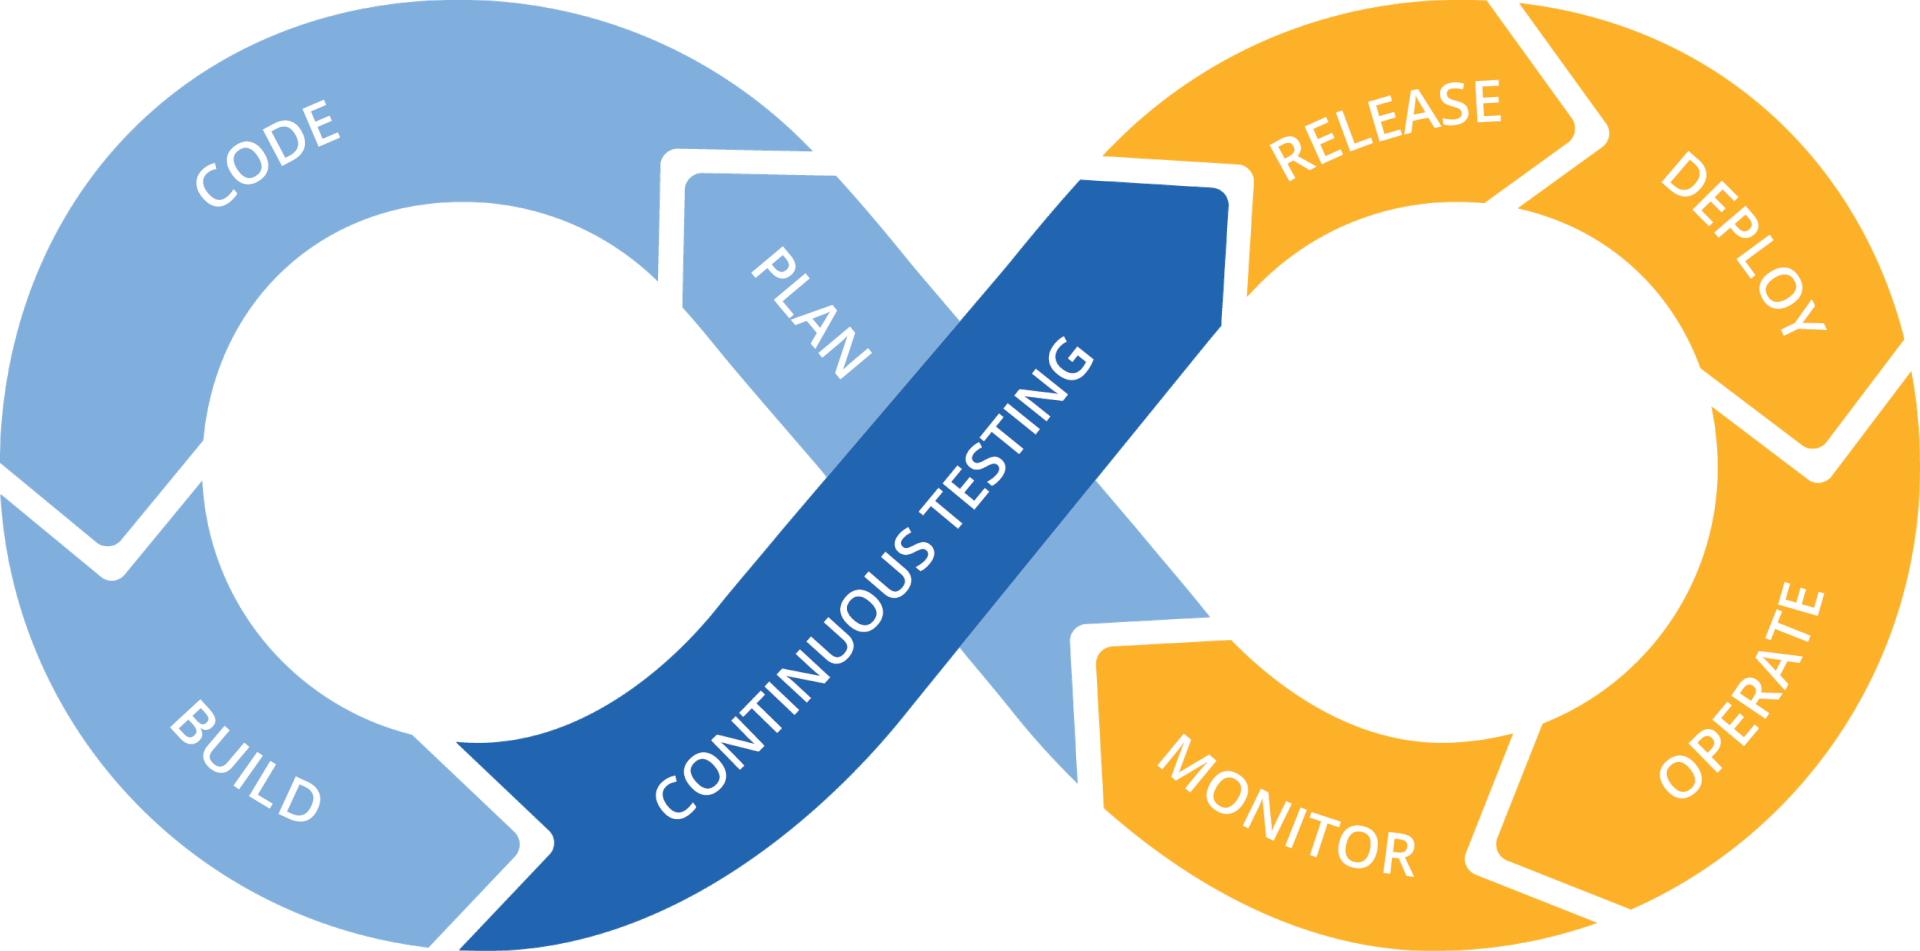
\includegraphics[width=1\textwidth]{Bilder/devopscycle}
	\caption{An example DevOpscycle}
	\label{fig:devopscycle}
\end{figure}